\chapter{Hashing}
Hashing is one of the approaches for efficient solving the dictionary and set representation problems. Various implementations differ in many ways but usage of a hash function and a fast table, typically represented by an array, is common to the most of them. Hash function transforms elements of universe into addresses of the table.

Represented sets are much smaller compared to the size of the universe. In order to prevent waste of space we are forced to use tables as small as possible. Typically size of the table storing the represented elements is chosen so that it is comparable to those of the hashed set. 

\begin{definition}[Load factor]
\label{definition-load-factor}
Let $n$ be the size of the represented set and $m$ be the size of the hash table storing the elements. Variable defined as \[ \alpha = \frac{n}{m} \] is called the load factor of the table.
\end{definition}

To formalise previous ideas load factors are typically kept in a predefined interval. In such case we are able to guarantee an overhead of the data structure.

Since the hash table is much smaller than the possible universe and arbitrary two elements can be represented they can share the same address after the hash function is used. This event is called a \emph{collision}. Very important for hashing is how collisions are handled. This is also the most interesting distinctive feature for different hashing models. In fact collision handling determines the time complexity of the scheme.

When two elements collide they are typically placed into a single \emph{bucket}. Bucket is often represented by the simplest data structure possible, for instance single linked list should be sufficient. In more sophisticated schemes, like perfect hashing, another hash table is used. 

So for imagination the find operation of a hash table works in the following way. Every element is given to a hash function as its argument. The element's address is then returned and used as an index for the hash table. Then we look into the bucket lying at the address if the element is stored inside or not.

If we represent buckets by singly linked lists the expected time of the find operation is proportional to the half of the length of the list.
\begin{lemma}
\label{lemma-expected-list-time}
Let $S$ be a set represented by a singly linked list. Moreover assume that for every element $x \in S$, $\Prob{x \text{ is argument of the find operation}} = \frac{1}{|S|}$. Then the expected time of the find operation is $\frac{|S| - 1}{2}$.
\end{lemma}
\begin{proof}
We compute expected time of the find operation directly from its definition. Let $x_i \in S$ be the $i$-th element of the list for $1 \leq i \leq |S|$. Time to find the element $x_i$ equals $i$. The expected time is then
\[
\begin{split}
\Expect{\text{Time of the find operation}} 
	& = \displaystyle\sum_{i = 1}^{|S|} i \Prob{x_i \text{ is the argument of the find operation}} \\
	& = \frac{\sum_{i = 1}^{|S|}{i}}{|S|} = \frac{|S|(|S| - 1)}{2 |S|} = \frac{|S| - 1}{2} \text{.}
\end{split}
\]
\end{proof}

As seen in the previous lemma the measure of time of an operation doest not have to be the worst case. Compare $|S|$ which is the worst case to the expected time $\frac{|S|}{2}$. Using just the worst case time does not tell much about the structure's behaviour. We are forced to use characteristics based on the probability that give more accurate results such as the expected operation's time. For hashing the difference means an asymptotic improvement.

\section{Assumptions of classic hashing}
In lemma \ref{lemma-expected-list-time} we computed the expected time of the find operation and used it as a measure of its time complexity. The computed expectation is based on the probability distribution of the input. We assumed its uniformity. In hashing similar situation occurs. If we want to calculate corresponding average results we need some assumptions on the probability of the input.
\begin{itemize}
\item Hash function $h$ distributes the elements of universe uniformly across the hash table.
\[
||h^{-1}(x)| - |h^{-1}(y)|| \leq 1 \text{ for every }x, y \in U \text{.}
\]
\item Every hashed set consisting of $n$ elements has the same probability of being represented among all the sets of the same size.
\[
\Prob{S \text{ is hashed}} = \frac{1}{\dbinom{|U|}{n}} \text{ for every set } S \subset U \text{ such that } |S| = n \text{.}
\]
\item Every element of the universe has the same probability of being an argument of an operation.
\[
\Prob{x \text{ is used as an argument of an operation}} = \frac{1}{|U|} \text{ for every } x \in U \text{.}
\]
\end{itemize}

These assumptions provides us with a probabilistic model for the average case analysis of classic hashing.

\section{Separate chaining}
Separate chaining may be considered the most basic hash table implementation. However it is sufficient for illustration of various problems, \cite{The-art-of-computer-programming}, \cite{DBLP:books/sp/Mehlhorn84} and \cite{DBLP:books/sp/MehlhornS2008}. Separate chaining usually utilises one hash function mapping elements of the universe to an address - an index of the array representing the hash table. Element is then stored in a bucket given by its hash address. Every bucket is represented by a singly linked list. 

Separate chaining, like the other classic models of hashing, is quite dependent on the hashed input. The assumptions we made are crucial for the average case analysis. For example consider hashing universe $U = \{0, \dots, N - 1\}$ for $N \in \mathbb{N}$ into a table of size $m \in \mathbb{N}$. Number $m$ is much smaller then $N$ and moreover it is chosen to be a prime. Primality of $m$ improves the uniformity of distribution of the hashed set across the hash table. 

\begin{figure}
  \centering
    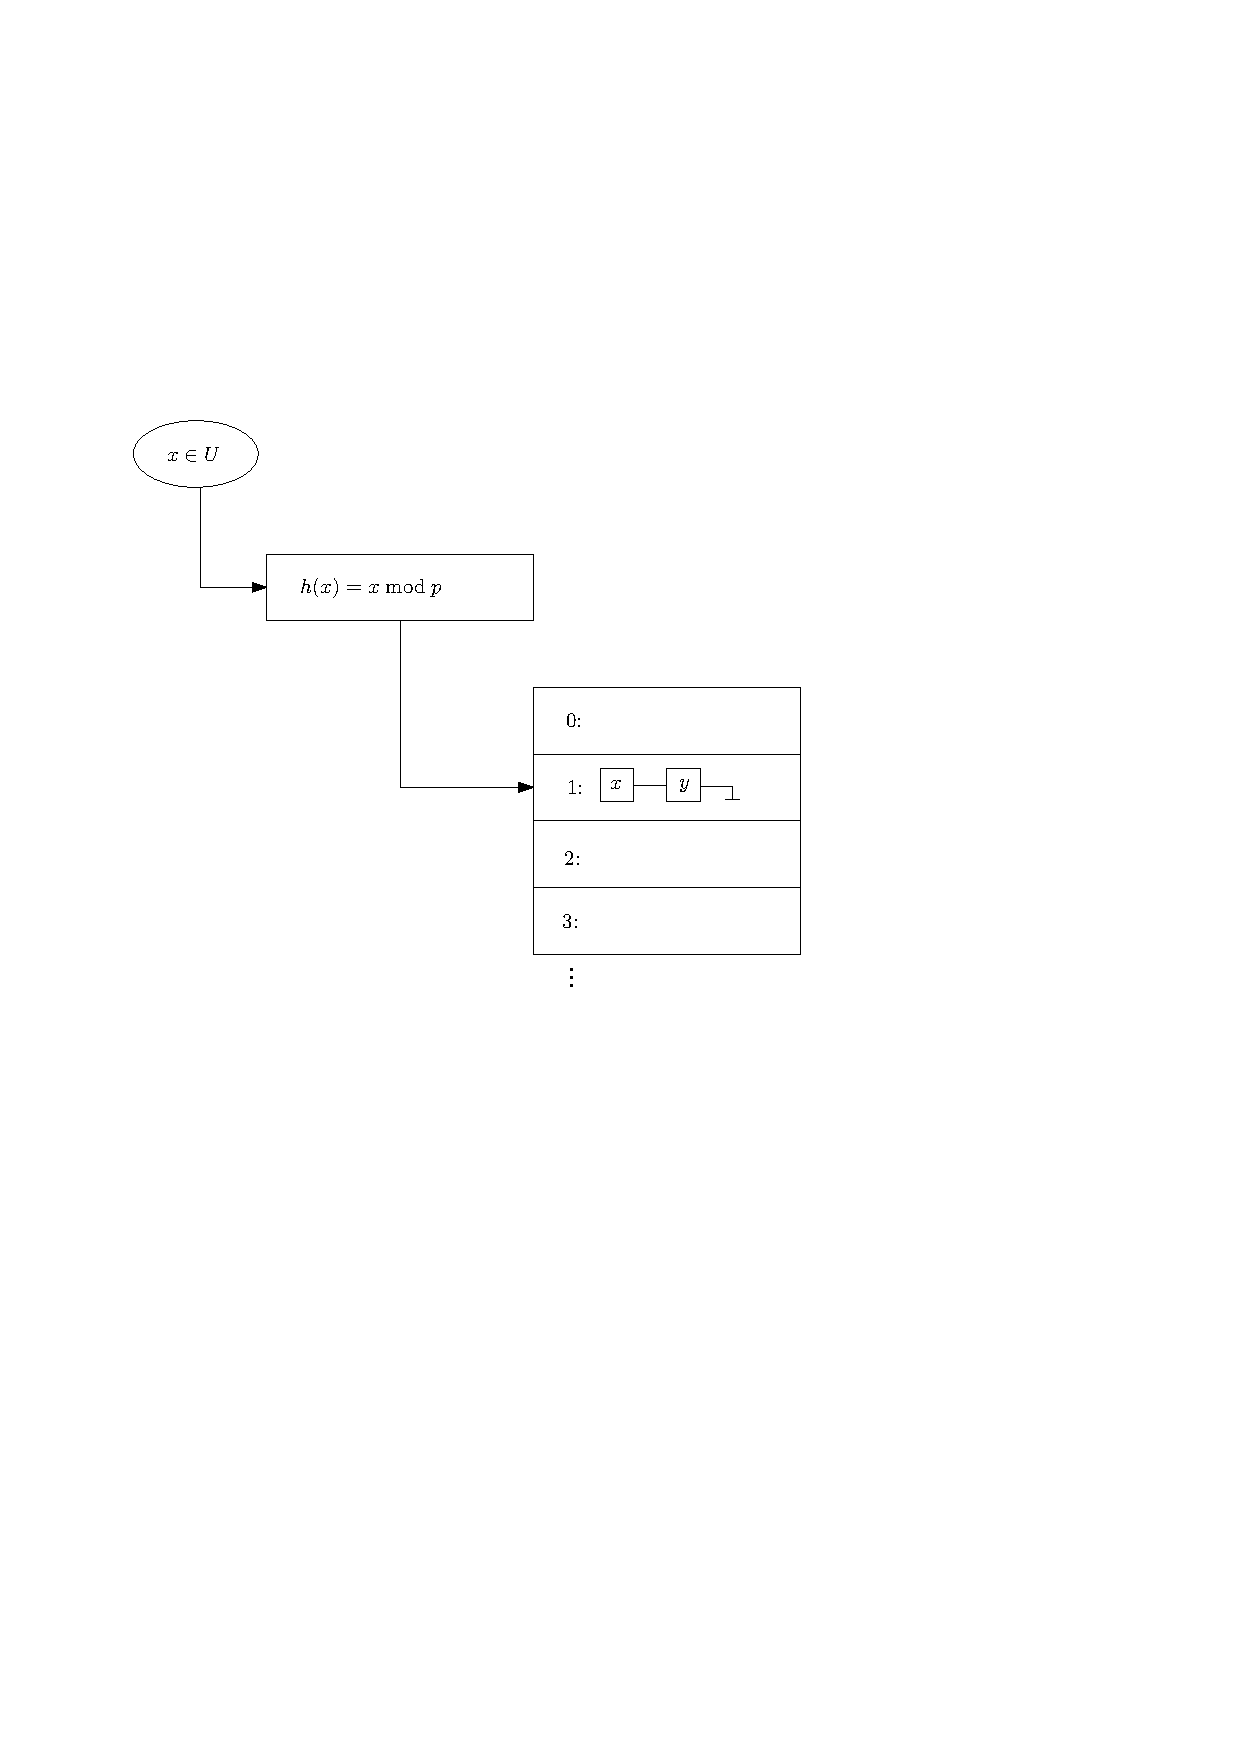
\includegraphics[width=0.5\textwidth]{images/hash_table}
  \caption{Concept of a hash table.}
\end{figure}

\begin{example}
Consider set $S = \{5n \setdelim n \in \{0, \dots, 5\} \}$ and table consisting of $10$ buckets. Set $S$ contains only 6 elements, so the table's load factor equals $0.6$. Function $x \bmod 10$ maps the elements just onto two addresses, $0$ and $5$. The table is clearly not used effectively. Choosing $m$ to be prime improves the results but is not a remedy.
\end{example}

The apparent disadvantage is that we use a single hash function known in advance. When the represented set, chosen by an adversary, is a subset of the preimage of a single bucket we run into problems. However our assumptions show that the probability of having such an input is quite low.

In order to illustrate how the model works the algorithms for separating chaining are presented. Although this model is quite simple the subroutines performing the operations on the singly linked lists are not discussed. They are understood as elementary operations. However they running times are proportional to the length of the represented chain. Notice that the insert procedure has to check if the element is already stored inside the list not to be stored twice. 

\begin{algorithm}
\caption{Find operation of the separate chaining.}
\label{algorithm-find-separate-chaining}
\floatname{algorithm}{Procedure}
\begin{algorithmic}
\REQUIRE $x \in U$
\STATE $h = h(x)$
\STATE
\IF {$T\left[h\right] \text{ contains } x$}
	\RETURN \textbf{true} \COMMENT{operation is successful}
\ELSE
	\RETURN \textbf{false} \COMMENT{operation is unsuccessful}
\ENDIF
\end{algorithmic}
\end{algorithm}

\begin{algorithm}
\caption{Insert operation of the separate chaining.}
\label{algorithm-insert-separate-chaining}
\floatname{algorithm}{Procedure}
\begin{algorithmic}
\REQUIRE $x \in U$
\STATE $h = h(x)$
\STATE
\IF {$T\left[h\right] \text{ doest not contain } x$}
	\STATE insert $x$ into chain $T[h]$
\ENDIF
\end{algorithmic}
\end{algorithm}

\begin{algorithm}
\caption{Delete operation of the separate chaining.}
\label{algorithm-delete-separate-chaining}
\floatname{algorithm}{Procedure}
\begin{algorithmic}
\REQUIRE $x \in U$
\STATE $h = h(x)$
\STATE
\IF {$T\left[h\right] \text{ contains } x$}
	\STATE remove $x$ from chain $T[h]$
\ENDIF
\end{algorithmic}
\end{algorithm}

\begin{theorem}[Average case of the separate chaining]
Let $U = \{0, \dots N - 1\}$ be the hashed universe where $N \in \mathbb{N}$. Let $S \subset U$ be the represented set and moreover $n = |S|$, $n \ll N$. Then the expected time of the successful find operation converges to $1 + \frac{\alpha}{2}$ and to $e^{-\alpha} + \alpha$ in the unsuccessful case.
\end{theorem}

\section{Coalesced hashing}
Collisions are solved by representing the chains of colliding elements directly stored in a hash table. 

\section{Open addressing}
Instead of having one pointer in the table we use secondary function for conflict resolution.
\subsection{Linear hashing}
\subsection{Double hashing}

\section{Universal hashing}
The basic idea of universal hashing is to remove the assumptions on uniformity of input from classic hashing.

\section{Modern approaches}
\subsection{Robin hood hashing}
\subsection{Cuckoo hashing}
\subsection{Hopscotch hashing}
This is a modification of linear hashing optimised for cache behaviour.

\section{Formalisms and notation}
In this section we describe notation and formalisms used to mathematically describe a hash table.

